\chapter{AI Design}
\label{chap:ai-design}

\section{Introduction}
Artificial Intelligence has transitioned from an experimental capability to a core component of modern productivity applications. In project management platforms, the integration of generative AI serves as a productivity multiplier rather than an autonomous replacement for human oversight. The role of AI in Nexus PM is to reduce the administrative overhead of task decomposition, metadata drafting, and project reporting.

By automating repetitive activities (such as breaking down project briefs into actionable checklists or compiling weekly status updates from task timelines), Nexus PM allows software engineering teams, product managers, and developers to focus on core execution. This chapter outlines the architecture, data flows, validation strategies, performance characteristics, and security parameters that define the AI subsystem.

\section{AI Architecture}
The AI subsystem uses a decoupled processing pipeline, sending requests asynchronously to external Large Language Models (LLMs) to prevent blocking main execution threads. Figure~\ref{fig:ai_architecture} illustrates the system context and runtime boundary configurations.

\begin{figure}[h!]
    \centering
    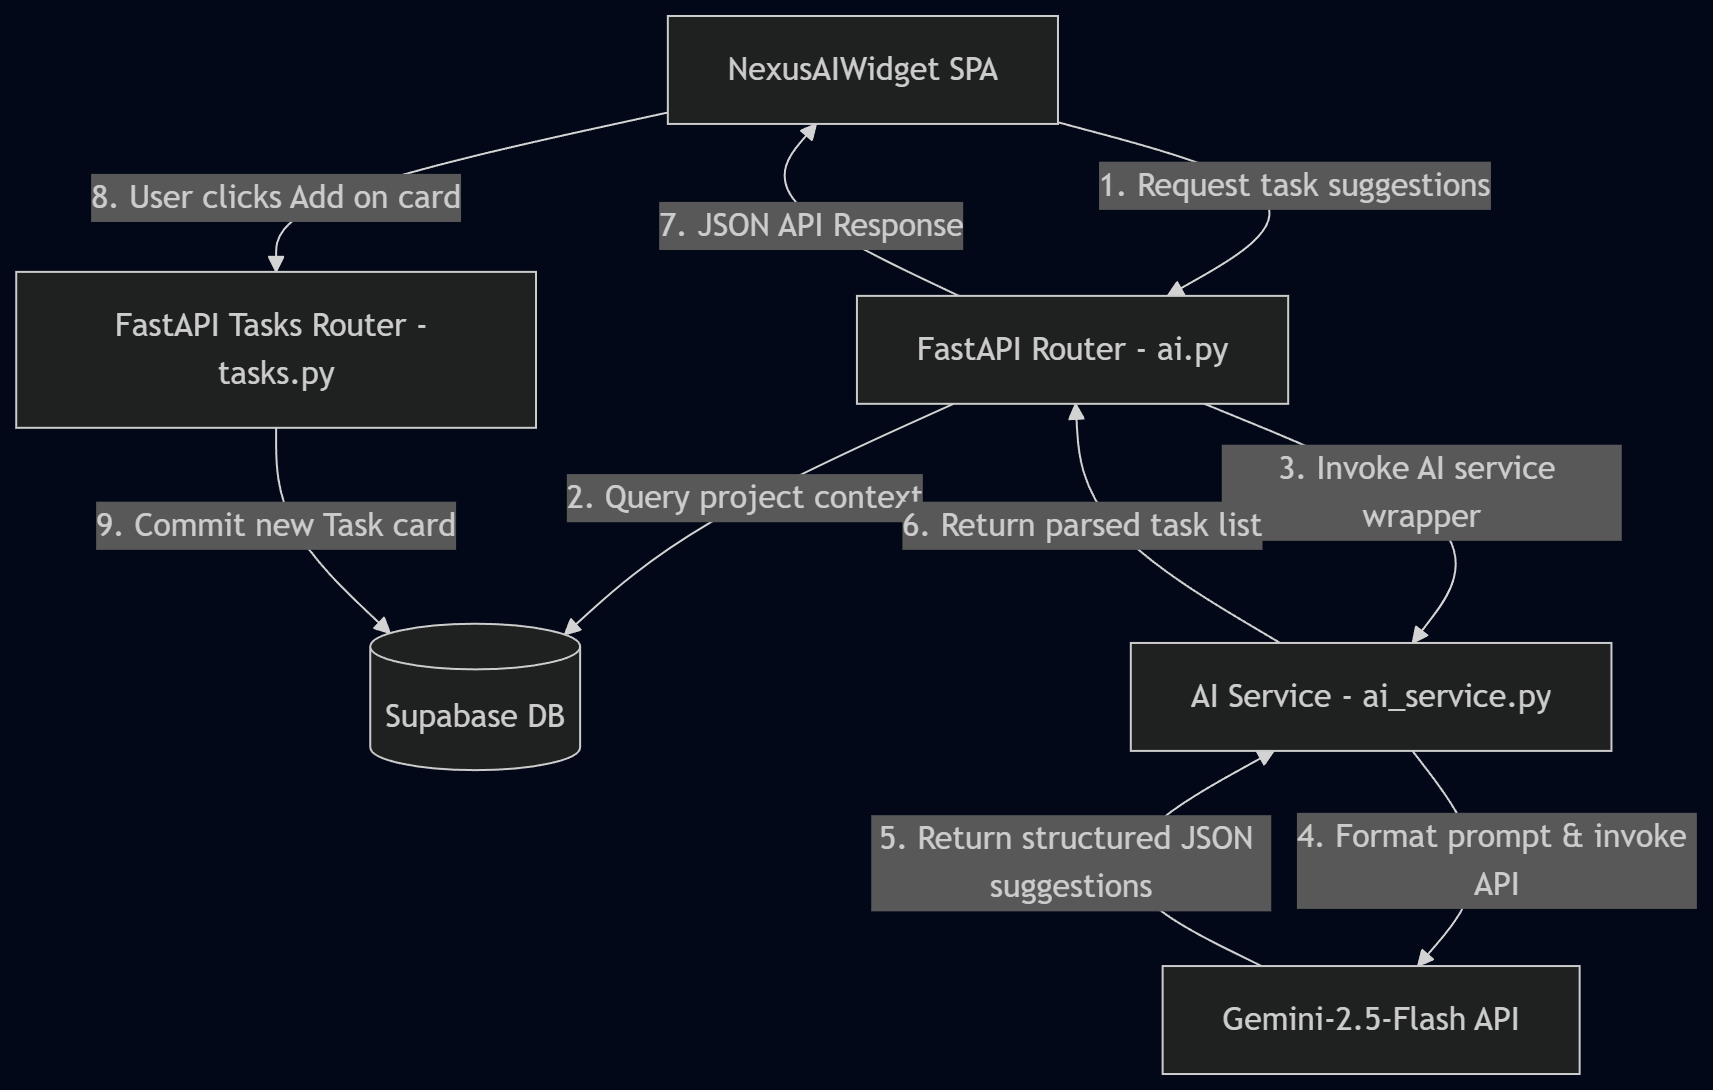
\includegraphics[width=\textwidth]{figures/ai-architecture.png}
    \caption{Nexus PM Asynchronous AI Subsystem and Data Flow Architecture}
    \label{fig:ai_architecture}
\end{figure}

The lifecycle of an AI request flows through several components:
\begin{enumerate}
    \item \textbf{Client Ingress:} The user initiates an AI action (e.g., requesting task suggestions) on the React client.
    \item \textbf{Context Aggregation:} The FastAPI backend receives the request, validates the project context, and queries the database for relevant metadata.
    \item \textbf{Prompt Assembly:} The prompt builder compiles project variables into formatted prompt templates.
    \item \textbf{LLM Execution:} The AI service dispatches the request to the Google Gemini 2.5 Flash API asynchronously over HTTPS.
    \item \textbf{Response Validation:} The response parser extracts the text block, validates the JSON format against Pydantic schemas, and commits the structured resources to the PostgreSQL database.
    \item \textbf{State Synchronization:} The client application is notified of the completed generation, updating the interface state.
\end{enumerate}

\section{AI Components}
The AI subsystem is composed of five logical components, summarized in Table~\ref{tab:ai_components}.

\begin{table}[h!]
\centering
\small
\renewcommand{\arraystretch}{1.4}
\begin{tabularx}{\textwidth}{l X}
    \toprule[1.5pt]
    \rowcolor{primary!5}
    \textbf{\color{primary}AI Component} & \textbf{\color{primary}Subsystem Responsibility} \\
    \midrule
    \textbf{GenAI Client} & Manages the lifecycle of connection pools to Google's API gateway over HTTPS, using API keys from system configurations. \\
    \textbf{Prompt Builder} & Compiles prompt templates, merges database variables, and sets system instructions. \\
    \textbf{Response Parser} & Isolates JSON string blocks from LLM responses, running regex cleanups to strip markdown code blocks. \\
    \textbf{Validation Engine} & Uses Pydantic models to validate structural type formats, preventing malformed data from being saved. \\
    \textbf{Error Handler} & Maps API timeouts, rate-limit failures, and gateway errors to clean application exceptions. \\
    \bottomrule[1.5pt]
\end{tabularx}
\caption{AI Subsystem Component Responsibilities}
\label{tab:ai_components}
\end{table}

\section{Current AI Features}
The platform implements four primary AI capabilities, detailed in Table~\ref{tab:implemented_ai_features}.

\begin{table}[h!]
\centering
\small
\renewcommand{\arraystretch}{1.4}
\begin{tabularx}{\textwidth}{l p{3.2cm} X}
    \toprule[1.5pt]
    \rowcolor{primary!5}
    \textbf{\color{primary}Feature Name} & \textbf{\color{primary}Backend Endpoint} & \textbf{\color{primary}Functional Workflow} \\
    \midrule
    Task Suggestions & \texttt{generate\_tasks\_from\_description} & Reads project description text, generates 5--7 actionable task suggestions, and returns them as a structured JSON array. \\
    Project Summaries & \texttt{summarize\_project} & Aggregates project descriptions, category metadata, and active task statuses to generate a text summary. \\
    Task Descriptions & \texttt{generate\_task\_description} & Accepts short task titles and context variables, generating detailed task descriptions. \\
    Meeting Minutes to Tasks & \texttt{meeting\_notes\_to\_tasks} & Parses raw meeting transcripts and notes, extracting actionable tasks and assigning estimated timelines. \\
    \bottomrule[1.5pt]
\end{tabularx}
\caption{Implemented AI Capabilities}
\label{tab:implemented_ai_features}
\end{table}

\section{Prompt Engineering Strategy}
To guarantee system stability, the platform uses a structured prompt engineering strategy:
\begin{itemize}
    \item \textbf{Role-Based System Instructions:} System prompts define the model's role (e.g., "You are a project management assistant") and output constraints (e.g., requesting raw JSON formatting).
    \item \textbf{Context Minimization:} The Prompt Builder includes only essential project metadata in request templates, minimizing token consumption and reducing processing latencies.
    \item \textbf{Structured Output Constraints:} Prompts define expected JSON schema parameters, including required fields, string lengths, and element counts, to ensure response consistency.
    \item \textbf{Deterministic Tuning:} Model configuration parameters (such as temperature) are tuned to ensure consistent, deterministic outputs across requests.
\end{itemize}

\section{Response Processing}
Since generative language models can occasionally return malformed responses, the backend implements a structured response validation workflow:
\begin{enumerate}
    \item \textbf{Markdown Cleanups:} The response parser strips markdown wrapper text (e.g., \texttt{```json ... ```}) to isolate raw JSON strings.
    \item \textbf{JSON Validation:} The cleaned response string is validated using Python's \texttt{json.loads}.
    \item \textbf{Pydantic Schema Validation:} The JSON object is parsed against Pydantic schemas (e.g., \texttt{TaskSuggestion}), verifying type constraints and field structures.
    \item \textbf{Sanitization Fallbacks:} If parsing or validation fails, the service logs the failure, attempts to extract partial fields, and falls back to a clean error response rather than committing malformed data.
\end{enumerate}

\section{Performance Considerations}
Integrating generative APIs introduces latency and rate limit challenges, which the platform manages using several optimizations:
\begin{itemize}
    \item \textbf{Asynchronous API Calls:} AI integrations use FastAPI's asynchronous support (\texttt{client.aio}), preventing API network latency from blocking the server's main request loop.
    \item \textbf{Rate-Limit Handling:} The service detects Gemini rate limits (HTTP 429), logging the event and returning user-friendly error messages to the client.
    \item \textbf{Cache Policies:} Analytical project summaries are cached in Upstash Redis, preventing redundant API calls when project data has not changed.
\end{itemize}

\section{Security and Privacy}
AI features are designed to protect user data and secure integration boundaries:
\begin{itemize}
    \item \textbf{Input Sanitization:} Input context is sanitized using Pydantic validation schemas to mitigate prompt injection risks.
    \item \textbf{Access Authorization:} Endpoints enforce workspace role checks (\texttt{require\_project\_role}), ensuring users can only run AI actions on projects they are member of.
    \item \textbf{Credential Isolation:} Gemini API keys are loaded via system environment variables, preventing exposure in client code or code repositories.
\end{itemize}

\section{Future AI Roadmap}
Future iterations of the platform plan to expand AI capabilities, as outlined in the roadmap in Table~\ref{tab:future_ai_roadmap}.

\begin{table}[h!]
\centering
\small
\renewcommand{\arraystretch}{1.4}
\begin{tabularx}{\textwidth}{l X}
    \toprule[1.5pt]
    \rowcolor{primary!5}
    \textbf{\color{primary}Roadmap Goal} & \textbf{\color{primary}Planned Capabilities} \\
    \midrule
    AI Sprint Planning & Automated velocity estimations, resource balancing recommendations, and milestone groupings based on historical sprint performance. \\
    AI Risk Analysis & Automated identification of blocking task dependencies, project delays, and timeline bottleneck predictions. \\
    AI Bug Prioritization & Classification of incoming bug reports based on stack traces, assigning priorities, and routing issues to specific developers. \\
    Natural Language Search & Semantic workspace search capabilities, letting users query project status using conversational queries. \\
    \bottomrule[1.5pt]
\end{tabularx}
\caption{Future AI Subsystem Development Roadmap}
\label{tab:future_ai_roadmap}
\end{table}

\section{Architectural Strengths}
The AI integration architecture delivers several key advantages:
\begin{itemize}
    \item \textbf{Structured Output Validation:} Validating AI responses against strict schemas ensures database integrity and prevents application parsing failures.
    \item \textbf{Low Operational Overhead:} Leveraging managed API services avoids the compute and maintenance costs of hosting local model engines.
    \item \textbf{Non-Blocking User Experience:} Asynchronous task execution ensures that the user interface remains active and responsive while generative processes run.
\end{itemize}

\section{Chapter Summary}
This chapter detailed the AI design of the Nexus PM platform, outlining the prompt engineering pipelines, validation strategies, performance configurations, and security boundaries. By using Google Gemini 2.5 Flash and enforcing structured JSON validation, the platform provides reliable AI capabilities while protecting workspace data. The next chapter will focus on the deployment architectures and operational topologies.
